\documentclass{article}
\usepackage[utf8]{inputenc}
\usepackage[margin=1.2in]{geometry}
\usepackage{mathtools}
\usepackage{enumerate}
\usepackage{natbib}
\usepackage{amssymb}
\usepackage{amsmath}
\usepackage[T1,T2A]{fontenc}
\usepackage[russian,english]{babel}
\selectlanguage{english}
\usepackage{multirow}

\title{Unsupervised Word Translation with Dutch and Russian}
\author{Svetlana Tchistiakova \& Guido Linders}
\date{\today}

\begin{document}

\maketitle
\section*{Introduction}
In the field of machine translation (MT), historically, high quality translation models are built using parallel corpora in a supervised way for parameter estimation, most recently and successfully with the help of neural networks (e.g. \citet{DBLP:journals/corr/WuSCLNMKCGMKSJL16}). However, certain language pairs (e.g. those involving low-resource languages), suffer from lack of parallel corpus data, making this infeasible \citep{nmt2017oestling}. Recent approaches have begun to use semi-supervised methods with combined parallel and monolingual corpora (e.g. \citet{DBLP:journals/corr/ChengXHHWSL16}). Those approaches only need a small amount of annotated data for training and thus are especially suited for language pairs for which very little parallel data is available.

% Parallel RU/NL corpus:
% https://github.com/ajinkyakulkarni14/TED-Multilingual-Parallel-Corpus

Another more recent approach in neural machine translation uses no parallel corpora at all but relies solely on monolingual embedding spaces that are then mapped to each other. This work can serve as the first step towards creating a larger MT system, not limited to only word translation (e.g. as produced by \citet{lample2017unsupervised}). In this project we create a word translation system for Russian and Dutch, following the method presented in \citet{conneau2017word}. This method follows a four-step process:

\begin{enumerate}
\item{Train monolingual word embeddings for each language from distributional data}
\item{Train a generative adversarial neural network (GAN) to find a mapping between source language embeddings as target language embeddings}
\item{Refine the parameters trained by the GAN using the Procrustus algorithm (symmetrically for source-to-target, and then target-to-source)}
\item{Calculate a similarity metric for a source language word to each target language word, and choose the best one as the translation}
\end{enumerate}

The word embedding \citep{rehureklrec}, GAN \citep{goodfellow2014generative}, and refinement/similarity calculation algorithms \citep{conneau2017word} that we use have all been described in detail by their source authors. We now seek to apply these algorithms to a new Dutch/Russian corpora. Where we have deviated from the method in \citet{conneau2017word} is primarily in the acquisition and processing of our corpus and the use of \texttt{gensim} \citep{rehureklrec} in training our word embeddings. 

In the rest of this report, we will cover (1) a slightly more in-depth explanation of the algorithm, (2) those implementation details which are particular to our approach, (3) an evaluation of the results, and (4) conclusion with suggestions for future work.

% Some papers on unsupervised MT
%https://arxiv.org/pdf/1710.11041.pdf
%https://arxiv.org/abs/1711.00043

\section{Explanation of the algorithm}
\label{algorithm}
The model as proposed by \cite{conneau2017word} consists of 3 steps, which are step 2-4 in the previous section. This algorithm starts with monolingual word embedding spaces in both the source and target language. In the first step a rough mapping from the the source language space to the target language space is estimated using a generative adversarial network. Effectively a rotation matrix is learned which maps the source language embedding space onto the target language embedding space. This network consists of a discriminator that tries to discriminate between the target language embedding and the source language embedding that is modified by the rotation matrix. The rotation matrix is trained to ``fool’’ the discriminator by trying to make the source and target embedding spaces as similar as possible so that the discriminator cannot distinguish between the two spaces. The training of the discriminator and rotation matrix is an iterative process.

In the next step this rotation matrix is refined by using the Procrustus algorithm on a subset of the embedding space, more specifically the most frequent words. The intuition is that the most frequent words have a more reliable representation in space because they have been seen more often in the training of the word embeddings. The Procrustus algorithm uses these most frequent words as anchor points and tries to minimize the distance between the closest anchor points using singular-value decomposition (SVD). This step can also be repeated for a certain number of iterations, but will have a very limited impact on the final performance after just one or two iterations

In the final step, actual word pairs are constructed. The most naive way of doing this is to match each source word with the K nearest neighbors in the target language space. This method, however, has the problem of being asymmetric in the sense that if a word in the source language is a nearest neighbor (NN) of a word in the target language space, the reverse does not have to be true. This leads to some source words being hubs, and having many NN’s in the target language space while other source words have no NN’s in the target language space. The authors propose another method where they compute, for each word in both the source and target language a mean similarity between the word and its K NN’s in the other language space. These mean similarities are then used to compute a similarity score between a word in the source language and a word in the target language. This final similarity score is called cross-domain similarity local scaling (CSLS). 


\section{Implementation details}

\subsection{Downloading comparable corpora}
For the training data, we wanted to create a comparable Russian/Dutch corpus, where each corpus covers similar topics, so that we can more effectively train word translations. Wikipedia contains a lot of data and is easily accessible. For it, we used the MediaWiki API to scrape Wikipedia. That is, we searched for random Wikipedia pages in the source language, and if that page contained a language link to the target language, we downloaded both pages. We alternated searching for Dutch pages first, and then searching for Russian pages first. In this way, we built up a comparable corpus consisting of the same number of documents on the same topics in each of the two languages. 

One problem with this approach is that each downloaded document might vary in number of words, which could happen if the Wikipedia articles in one language are generally less descriptive than in the other. This was one problem we did not address in our work. Another potential problem with data from Wikipedia is that it contains a relatively high number of proper nouns. We can work around this problem by increasing the number of documents and by using a cut-off threshold for the number of types as well as a minimum number of occurrences of a word to be included in the word embeddings. 

\subsection{Data processing}

We processed the data by splitting the text documents into sentences, normalizing the sentences, and splitting them into lists of words. Normalization included removing punctuation, converting each sentence into lower case, simplifying numeric expressions, and lemmatization.

The text data was split into sentences using the Python3 \texttt{NLTK} package \citep{bird2009natural}, and then converted into lower case. Numeric expressions were replaced with a single type called \texttt{NUM}. This was done in order to avoid having a potentially infinite number of word embeddings representing numeric expressions. Note that we did not replace any numbers that were already written out in words with \texttt{NUM}, though this is another normalization that could be tried. 

Since we are focused on word translation, we are particularly interested in the semantic space, and less interested in syntactic differences of word forms. (The opposite may be true in a larger project focused on sentence translation.) Russian, in particular, exhibits a rich inflectional morphology, which results in many different word forms for the same semantic concept, and could needlessly increase the number of word embeddings in our model. For these reasons we chose to try experiments in which we lemmatize the corpus before training word embeddings, in addition to experiments without lemmatization. Lemmatization was performed both before training of the language-specific word embeddings, as well as to create the Dutch-Russian/Russian-Dutch evaluation dictionaries. One potential problem with lemmatization is that it introduces another source for errors, in case a wrong lemma is chosen. This could in turn negatively impact the performance of the model.  

To perform Russian lemmatization, we used the \texttt{pymystem3} tool\footnote{Code retrieved from: https://github.com/nlpub/pymystem3}, which is a wrapper around the Yandex Mystem 3.0 tool \citep{segalovich2003fast}. Lemmatization was performed on a per-sentence level. 

For Dutch, we used the freely available CSTLemmatizer tool\footnote{Code retrieved from: https://github.com/kuhumcst/cstlemma.} \citep{jongejan2009automatic}. Because of the slow nature of invoking this tool from our program, lemmatization of Dutch was performed on whole documents, before sentence splitting. For some Dutch words the lemmatizer generates more than one lemma. In this case, the first lemma was chosen for normalization to train word embeddings, and all lemmas produced were used as entries in the evaluation dictionary. Ideally we would like to use the context of the word for deciding which lemma to use. A part-of-speech (POS) tagger might help with this as the different lemmas often have a different POS tag. However the Dutch lemmatizer does not provide the POS tag with the different lemmas. For this reason we have left the step of inferring the correct lemma for Dutch from the context and its POS for future work. When creating the evaluation dictionaries, we do not have any information on the POS tag because there are no surrounding words for context. In future work, the POS tag might be able to be inferred from the English word in the original dictionaries, or using a morphological analysis tool. 

\subsection{Generating word embeddings}

The Python3 \texttt{gensim} \citep{rehureklrec} library was used to generate word embeddings. The normalized, lemmatized sentences were fed directly into the \texttt{gensim} \texttt{Word2Vec} model, which trained language-specific word vectors for Dutch and for Russian. The number of word tokens (i.e. length of the corpus in words) and the vocabulary size (unique word tokens) for each language can be found in Table \ref{table:word-count}. We did not limit the vocabulary size for the word vectors as we could limit this at a later stage in the model of \cite{conneau2017word}. 

\begin{table}[ht]
\centering
\begin{tabular}{|l|l|l|l|l|}
\hline
        & & \textbf{Documents}     & \textbf{Word tokens} & \textbf{Vocab size} \\ \hline
\textbf{Dutch}       & Lemma & 70275   & 127,320,984      & 29,786      \\ \hline
        & No lemma   & 70275           & 127,627,062      & 30,251      \\ \hline
\textbf{Russian}     & lemma & 70275   & 198,561,330      & 38,681      \\ \hline
        & No lemma   & 70275           & 190,516,290      & 27,714      \\ \hline
\end{tabular}
\caption{Number of words used for training language-specific word vectors. The ``lemma'' row indicates that the input text was lemmatized prior to training word embeddings, whereas the ``no lemma'' row was not.}
\label{table:word-count}
\end{table}

For the generation of the word vectors we used continuous bag-of-words (CBOW). This technique uses a limited number of context words in generating word representations. In our case we used the default window of 5. We chose CBOW over Skip-gram because it has a faster training time and the accuracy for most frequent words is slightly better \citep{mikolov2013efficient}. In line with \citet{conneau2017word} we used 300 as our word embedding size. Finally, we sorted the word embeddings on frequency so that we could later limit our vocabulary size by cutting off the least frequent words. For the other parameters we mostly used default values and for these details we refer to our implementation\footnote{See \texttt{w2vconfig.py} in our code for these details.}.

\subsection{Training the model}
The word vectors were then directly fed into the model of \cite{conneau2017word}\footnote{Code retrieved from: https://github.com/facebookresearch/MUSE.}. As this model is fully unsupervised, it does not need any gold-standard dictionaries for creating the translation pairs. However the actual implementation needs a small dictionary which is used for intermediate evaluation and, after analyzing the code, it does not seem that the implementation uses these dictionaries to facilitate learning of the translation pairs, for example in choosing the best rotation matrix from a set of rotation matrices.

To choose the hyperparameters, we did some experiments with different settings. However as the model takes some time to finish we were limited in doing a lot of experimenting. Therefore most parameters were set to values as described by \citet{conneau2017word} or were kept to default values. We'll discuss the most important settings below. For other parameter settings we refer to our implementation\footnote{See train.sh as well as \texttt{unsupervised.py} in the folder \texttt{MUSE} for details on the parameter settings}.

We used a vocabulary size of 35000. This was about the maximum we could use as our own word embeddings generated around 35000 lemmas. This means we hardly removed low frequent words which could have a negative impact on the results as those words have not been seen a lot in training the word embeddings and might be wrongly represented. Please note that we did exclude words with a frequency of less than 5 in the training of the word embeddings However, since we use data from Wikipedia, probably there are still a lot of proper nouns in these embeddings. The reason for not filtering out more words is that our vocabulary size is already relatively small and we did not want to make it even smaller. 

For the discriminator, we used the details as described by \citet{conneau2017word}. The discriminator has 2 hidden layers of size 2048. In contrast to \citet{conneau2017word}, all of the words are used in the discriminator. Adversarial learning is done with 5 epochs and each epoch consists of 100,000 iterations as around those numbers the discriminator loss stabilizes and we want to prevent the model from overfitting the data, which could have a negative impact on the results. Finally, a batch size of 32 is used and optimization is done using stochastic gradient descent. 


\section{Evaluation}
\subsection{Method}
For language pairs with little to no parallel corpora there are often also no word translation dictionaries available. Indeed, for our language pair we could not find a high quality, freely available dictionary. As such, we bootstrapped from the English/Dutch and English/Russian dictionaries provided by \citet{conneau2017word} to create a two-way dictionary of Dutch and Russian in order to evaluate the words translations that come out of our model. We thus use English as an intermediate language to generate word translation pairs of Dutch/Russian. These dictionaries are of high quality, and sorted by word frequency. However, they contain many polysemous words, that is, an English word typically has a few different translations into the target language, some of which express very different semantic senses. We matched the two dictionaries up by creating a many-to-many mapping between the Dutch and Russian words which had the same English translation. This means we get the same word pairs for both directions of translating. See Figure \ref{many_mapping} one for a visualization.

\begin{figure}
\centering
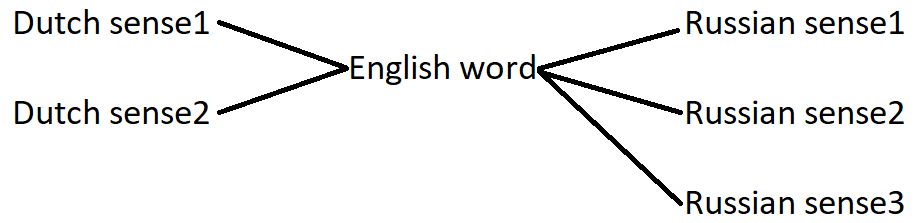
\includegraphics[scale=0.4]{many_mapping.png}
\caption{We generate a many-to-many mapping between each Dutch translation of an English word and each Russian translation of the same English word. In this example the English word has two different senses in Dutch and three different senses in Russian.}
\label{many_mapping}
\end{figure}

This method causes difficulties in the case of English words which may contain multiple unrelated senses in Dutch and/or Russian. For example, the English word ``iron'' out of context is ambiguous in the meaning of ``object to straighten clothes'' and ``the metal.'' Dutch and Russian both use two separate words in these contexts, as depicted in Table 2. Using the English word as a base, and without any other context, we cannot discern which words in Russian and Dutch correspond to one another. Since we simply create a many-to-many mapping between all the Dutch words and all the Russian words under the same English headword, for example, the Dutch word ``Strijkijzer'' will be incorrectly translated into Russian as both ``утюг'' and ``железо''. 

\begin{table}[ht]
\centering
\label{table:iron}
\begin{tabular}{|l|l|l|}
\hline
        & Object to straighten clothes & Metal                  \\ \hline
English & iron                         & iron                       \\ \hline
Dutch   & strijkijzer                  & ijzer                      \\ \hline
Russian & утюг    					   & железо \\ \hline
\end{tabular}
\caption{English polysemous word ``iron'' with separate words in Dutch/Russian}
\end{table}

Another problem is that no word translation model (supervised and unsupervised) has been evaluated on our language pair. This makes it very difficult to compare the results of our approach to other models or even a simple baseline. For this reason we decided to compare the results of training on our own word embeddings with training on the FastText \citep{bojanowski2016enriching}Wikipedia word embeddings, the same ones used by \citet{conneau2017word}.

Our evaluation method uses the same CSLS and nearest neighbours (NN) metrics as \citet{conneau2017word} and as explained in Section \ref{algorithm}, using our bootstrapped Dutch/Russian dictionary. These resulting dictionaries could provide an overly optimistic estimate of performance. That is because, for example, if the model translates the Dutch word ``Strijkijzer'' into the unrelated Russian word ``железо,'' the accuracy metric would incorrectly report this as a correct translation.

Note that the \texttt{MUSE} code from \citet{conneau2017word} uses a small subset of the dictionary to test during the Procrustes refinement step for memory and speed reasons. For this portion, we also created a smaller dictionary, in which we removed polysemous words by simply choosing the first available translation.

The source code from \citet{conneau2017word} also comes with an evaluation script, which we used in evaluating the performance of our model. The reason for using this evaluation script is to use the same steps in the evaluation as in \citep{conneau2017word} and to be able to compare our results with theirs, even though the language pairs differ. As Dutch and English are relatively similar we would expect the results on Dutch-Russian to be comparable to results on English-Russian as well as in the other translation direction. 

\subsection{Results}

Unfortunately, we ran into some problems during model training using the \texttt{MUSE} code from \citet{conneau2017word} that seemed to have prohibited us from getting proper working results. Because \citet{conneau2017word} have reported results on an English/Russian set, we decided to choose this as a baseline model to run through their code. We used this language pair as a baseline to make sure that our system is working correctly and also because we would expect similar results to the Dutch/Russian set as the languages share relatively a lot of similarities in semantics- and morphology-wise. We used the same fastText vectors that they report using, although some of our hyperparameters had to be lowered in order to allow running on the hardware available to us. 

As reported in Table 3, the performance of the Russian $\rightarrow$ English model seems very good. However, the results on English $\rightarrow$ Russian are near 0, as are the results on all other combinations of Dutch/Russian with and with fastText vectors and with our own vectors, with and without lemmatization (where applicable). Since we would expect the English $\rightarrow$ Russian direction with the fastText vectors to have a performance of better than 0, we suspect that either something in their code, in our set up or in the parameter settings of the model has gone wrong. Unfortunately, we were not able to resolve these issues. This is partly due to the fact that training the model is time-consuming. In addition, the problem of overlaying 2 vector spaces without supervision may have many local optima, and it's possible that without the right initialization and parameter settings, the model is entirely unable to converge. 

\begin{table}[ht]
\centering
\label{table:results}
\begin{tabular}{|l|l|l|l|l|l|l|l|}
\hline
\multicolumn{2}{|l|}{\multirow{2}{*}{}}   & \multicolumn{2}{l|}{\textbf{NL $\rightarrow$ RU}} & \multicolumn{2}{l|}{\textbf{RU $\rightarrow$ NL}} & \textbf{EN $\rightarrow$ RU} & \textbf{RU $\rightarrow$ EN} \\ \cline{3-8} 
\multicolumn{2}{|l|}{}                    & Lemma         & No lemma    & Lemma & No lemma   & \textbf{-}   & \textbf{-}     \\ \hline
\multirow{2}{*}{\textbf{fastText}} & NN   & -             &   0.11      &  -    &  0.75      &    0.09      &    62.86       \\ \cline{2-8} 
                                   & CSLS & -             &   0.22      &  -    &  0.65      &    0.09      &    65.91       \\ \hline
\multirow{2}{*}{\textbf{ours}}     & NN   &  0.00         &  0.00       & 0.00  &  0.00      & -            & -              \\ \cline{2-8} 
                                   & CSLS &  0.00         &  0.00       & 0.00  &    0.13    & -            & -              \\ \hline
\end{tabular}
\caption{NN and CSLS metric results (for K=1) on our own vectors created from the Wikipedia data, as compared to the fastText baselines from \texttt{MUSE}. The ``lemma'' column indicates that the input text was lemmatized prior to training word embeddings, whereas the ``no lemma'' column was not (only relevant for our vectors). The English/Russian models were also trained as a baseline to make sure the original system words as it should. Unfortunately, an error in either the code or our set up or a wrong parameter setting has prevented us from getting proper results.}
\end{table}


\section{Conclusion}
For now there is, unfortunately, very little to conclude as we did not get the model to work correctly. We still think that, once we are able to resolve the issues with the model, our results would be relatively close to the English/Russian set. However because we used a much smaller data size in generating the word embeddings and our data probably still contains a lot of proper nouns, we expect our performance to be a bit lower. We also expect a positive influence on using lemmatization, even though it introduces another potential source for errors. 

For future work (assuming issues with the model can be resolved) the first step could be to download significantly more data from Wikipedia that would generate larger word embeddings (with more lemmas) and train these word embeddings on the model. With more data our word embeddings would become more accurate in representing the semantics of the word and would contain a relatively lower percentage of proper nouns. A second step could be to see if we can tune the parameters better to overlap the Dutch and Russian embeddings better and obtain better translation pairs. For this we could extract and analyze the word pairs that come out of the model. 

Also work on the Dutch and Russian lemmatizer could be done to improve the quality of the generated lemmas, which could facilitate performance of the model as well. As mentioned previously we could try to predict the Part-of-Speech (POS) tag for the word, given the context words. This in turn might guide us in choosing the correct lemma. 

Future work could improve the gold-standard dictionary for evaluation that was created manually and contains word pairs that are not translations of each other. Future work could also look at improving methods for creating word translation dictionaries for language pairs for which there are no word translation dictionaries available. One could try to improve the method we used by using an intermediate language. As explained this method has its limits, especially for polysemous words and could be improved. 

% REFERENCES
\bibliographystyle{apalike}
\bibliography{references}

\end{document}
